% ===========================================================
% co2_credits.tex
% Carbon-credit implications of per-bus, per-quarter marginal
% emission factors produced by \cenpipe{} / cen2gtopt.
% ===========================================================
\section{Carbon-Credit Implications}
\label{sec:credits}

A per-bus, per-quarter marginal emission factor
$\varepsilon^{\mathrm{bus}}_{b,t}$ is not only a research artefact; it
is also the formal input expected by an entire family of voluntary and
compliance carbon-crediting standards.  This section catalogues those
standards (Sec.~\ref{sec:credits-lit}), maps the
\texttt{cen2gtopt} output schema onto each one
(Sec.~\ref{sec:credits-ops}), reports a worked example for a
hypothetical 100~MW photovoltaic plant at the CRUCERO 220~kV bus on
2026-04-22 (Sec.~\ref{sec:credits-worked}), and closes with the
limitations and forward agenda
(Sec.~\ref{sec:credits-limits}).

\subsection{Marginal-Emission Methodologies in Voluntary Carbon Markets}
\label{sec:credits-lit}

The Clean Development Mechanism (CDM) under the Kyoto Protocol
established the canonical decomposition of a grid emission factor
into an Operating Margin (OM), a Build Margin (BM), and a Combined
Margin
$\mathrm{CM}=\tfrac{1}{2}\mathrm{OM}+\tfrac{1}{2}\mathrm{BM}$ in
\textit{Tool~07: Tool to calculate the emission factor for an
electricity system}~\cite{UNFCCCTool07}.  The OM is intended as a
\emph{short-run displacement} factor for renewable-electricity
projects and admits four computation variants: simple~OM,
simple-adjusted~OM, dispatch-data analysis~(OM-DDA), and average~OM.
The OM-DDA variant requires per-unit hourly dispatch and yields the
most defensible short-run displacement signal — exactly the level of
granularity at which Coordinador El\'ectrico Nacional (CEN)
publishes the underlying inputs.  Tool~07 underpins
AM0103~\cite{UNFCCCAM0103}, ACM0002~\cite{UNFCCCACM0002}, and the
small-scale methodologies AMS-I.D.\ and
AMS-I.F.~\cite{UNFCCCAMSID,UNFCCCAMSIF}.

Verra Verified Carbon Standard (VCS) v4.5~\cite{VerraVCS45}
inherits Tool~07 by reference for grid-renewable methodologies via
its VMR (Verra Methodology Revision) bridge documents and
VMR0007~\cite{VMR0007}.  The Gold Standard for the Global Goals
\textit{Renewable Energy Activity Requirements}~\cite{GSRENEAR}
adopts a simplified-OM variant for projects in least-developed-country
grids; for Chile, full Tool~07 OM-DDA is preferred.  None of these
voluntary-market methodologies currently publish an endorsement of
quarter-hourly granularity; all stop at the hourly level.

A second family of standards, originating in the corporate scope-2
accounting context, operates strictly on a time-matched
\textit{hourly} basis.  The Greenhouse Gas Protocol Scope~2 Quality
Criteria~\cite{GHGScope2} introduced market-based scope-2 reporting in
2015; the EnergyTag Granular Certificate (GC) Standard
v2~\cite{EnergyTagGC} formalised hourly Energy Attribute Certificates
in 2024; the 24/7 Carbon-Free Energy Compact~\cite{CFE247} and
RE100's 2024 hourly-matching update~\cite{RE100Hourly} push the same
agenda.  All four require hourly per-MWh emission factors as their
denominator; the per-quarter $\varepsilon^{\mathrm{bus}}_{b,t}$
produced by \cenpipe{} is a strict refinement.

The successor to the CDM under Article~6.4 of the Paris Agreement is
the Sustainable Development Mechanism (SBM), whose 2024 4DM Working
Group draft~\cite{Article64Draft} explicitly contemplates
\emph{hourly accounting} as one of the supported additionality
methodologies for Emission Reduction~(ER) credits.  The integrand
$\sum_t \varepsilon_t \cdot \Delta E_t$ — project energy times
hourly counterfactual emission factor — is, almost verbatim, the
formal definition of an ER unit in the draft text.

Finally, on the regulatory side, the EU Carbon Border Adjustment
Mechanism (CBAM)~\cite{CBAM2023} for embedded electricity emissions
of imported goods presently uses an annual default factor; the
implementing acts foreshadow a transition to country-specific and
later subnational marginal factors as data infrastructure matures.
California's Renewables Portfolio Standard / Resource
Adequacy~\cite{CARPSRA} and the Tradable REC programme provide a
locational-plus-temporal precedent at compliance scale.
Table~\ref{tab:credits-methodology} summarises the granularity,
dispatch-data requirements, and Chilean applicability of each
methodology.

\begin{table}[t]
\centering
\caption{Carbon-credit methodologies and their granularity in space,
time, and dispatch-data requirements.  ``A'' annual, ``M'' monthly,
``H'' hourly, ``Q'' quarter-hourly.  ``Loc.''~indicates whether the
methodology supports per-bus differentiation.}
\label{tab:credits-methodology}
% credits_methodology_compare.tex
% Comparison of carbon-credit methodologies that consume an electric-grid
% emission factor.  Granularity: A = annual, M = monthly, H = hourly,
% Q = 15-minute.  Dispatch-data?: whether the methodology requires
% per-unit dispatch (vs.\ system aggregates).  Hourly?: whether the
% methodology supports time-matched crediting.  Locational?: whether the
% methodology supports per-bus differentiation.  Chile?: applicability
% under the current SEN regulatory framework.
\setlength{\tabcolsep}{4pt}
\renewcommand{\arraystretch}{1.05}
\footnotesize
\begin{tabular}{@{}p{0.34\linewidth}cccccc@{}}
\toprule
Methodology / standard & Year &
  Gran. & Disp.\ data & Hourly & Loc.\ & Chile \\
\midrule
CDM Tool~07 v07.0 — OM/BM/CM             & 2018 & A & no  & no  & no  & yes\\
CDM Tool~07 OM-DDA variant               & 2018 & H & yes & yes & no  & yes\\
CDM AMS-I.D./AMS-I.F.\ (small-scale RE)  & 2022 & A & no  & no  & no  & yes\\
CDM AM0103 (RE for grid $>$15 MW)        & 2018 & A & no  & no  & no  & yes\\
CDM ACM0002 (large-scale grid RE)        & 2020 & A & no  & no  & no  & yes\\
Verra VCS v4.5 / VMR0007 (RECs revised)  & 2024 & A & no  & no  & no  & yes\\
Gold Standard RE-AR (LDC simplified-OM)  & 2023 & A & no  & no  & no  & yes\\
Article~6.4 SBM draft (4DM hourly)       & 2024 & H & yes & yes & opt & yes$^\ast$\\
GHG-Protocol Scope~2 Quality Criteria    & 2015 & A & no  & no  & no  & yes\\
EnergyTag GC Standard v2                 & 2024 & H & yes & yes & yes & yes$^\ast$\\
24/7 CFE Compact (UN-Energy)             & 2021 & H & yes & yes & yes & yes$^\ast$\\
RE100 Hourly Matching (2024 update)      & 2024 & H & yes & yes & yes & yes$^\ast$\\
EU CBAM Reg.\ 2023/956 (embedded elec.)  & 2023 & A & no  & no  & no  & exp.\\
\bottomrule
\end{tabular}

% $^\ast$ Article 6.4, EnergyTag, 24/7 CFE, and RE100 Hourly are all
% applicable in principle to Chile but do not yet have a designated
% national operator for issuance and tracking; the present pipeline
% would furnish their hourly/locational emission-factor input.

\end{table}

\subsection{Operationalising per-bus marginal factors}
\label{sec:credits-ops}

Three distinct uses of $\varepsilon^{\mathrm{bus}}_{b,t}$ are
considered, each tied to a different methodology family.

\paragraph{Operating Margin under CDM Tool~07 OM-DDA}
The OM-DDA variant of Tool~07 requires the hourly dispatch of each
generator $g$ and a fuel-attributed emission factor
$\varepsilon_{f(g)}$.  The 96-quarter granularity of \cenpipe{}
strictly subsumes Tool~07's hourly granularity; the OM is therefore
constructed as the dispatch-weighted mean over fossil units only,
\begin{equation}
\mathrm{OM}^{\mathrm{DDA}} =
  \frac{\sum_{g\in\setG_{\mathrm{fos}}} \sum_t
        \varepsilon_{f(g)}\,p_{g,t}}
       {\sum_{g\in\setG_{\mathrm{fos}}} \sum_t p_{g,t}},
\label{eq:om-dda}
\end{equation}
which the published cen2gtopt parquet exposes directly through the
\texttt{epsilon\_at\_bus} column once the hydro-and-renewable rows
($\varepsilon=0$) are filtered out.  Because Tool~07 explicitly
permits hourly dispatch data, the move to quarter-hourly does not
require a methodology revision; the auditor records the source
granularity in the project design document and aggregates upward.

\paragraph{Hourly Article~6.4 ER credits}
For Article~6.4 ER crediting of a renewable project that displaces
energy at bus $b$, the issued ER volume per period is
\begin{equation}
\mathrm{ER}_{b,t} =
  \varepsilon^{\mathrm{bus}}_{b,t} \cdot \Delta E_{b,t},
\label{eq:er-art64}
\end{equation}
where $\Delta E_{b,t}$ is the project's metered injection at bus $b$
in period $t$.  The published parquet provides
$\varepsilon^{\mathrm{bus}}_{b,t}$ at exactly the granularity that
the 4DM draft text references.  The same integrand applies at hourly
or quarter-hourly resolution; aggregation to either is a downstream
choice of the issuance registry.

\paragraph{EAC time-matching for grid-charged BESS}
Grid-charged battery energy storage systems pose an open question
under most VCS methodologies: a BESS that charges from a
high-$\varepsilon$ bus and discharges at a low-$\varepsilon$ hour
generates negative net abatement, while one that times its charging
to low-$\varepsilon$ hours and discharges at high-$\varepsilon$ hours
delivers a substantial positive abatement.  Existing methodologies
either ignore the temporal correlation or apply a constant grid
factor.  The per-quarter $\varepsilon^{\mathrm{bus}}_{b,t}$ enables
the natural extension
\begin{equation}
\mathrm{ER}^{\mathrm{BESS}}_b =
  \sum_t \varepsilon^{\mathrm{bus}}_{b,t}
         \bigl(P^{\mathrm{dis}}_{b,t} - P^{\mathrm{ch}}_{b,t}\bigr),
\label{eq:er-bess}
\end{equation}
which the present authors advocate as the correct accounting basis
for storage in a future revision of VCS / Article~6.4 methodologies.
Section~\ref{sec:bess} (the northern-bus business case) shows that
this expression is the same integrand the project developer
maximises in the dispatch optimisation.

\paragraph{EnergyTag and 24/7 CFE matching}
EnergyTag GC and the 24/7 CFE Compact require an hourly emission
factor at the consumer's grid node.  The
\texttt{epsilon\_at\_bus\_pid} column of the cen2gtopt output (the
PLEXOS-PID-corrected variant) is a drop-in input for both standards
and is directly comparable to PJM's Locational Marginal Emissions
feed~\cite{PJMLME2024}.

\subsection{Worked Example: 100~MW Hypothetical PV at CRUCERO}
\label{sec:credits-worked}

To quantify the difference between the three accounting variants
identified above, a hypothetical 100~MW photovoltaic plant is sited
at the CRUCERO 220~kV bus — the same northern transmission bus
analysed in the BESS business case of Sec.~\ref{sec:bess} — for the
operating day 2026-04-22.  The plant's hourly capacity factor is
modelled as a clipped raised-cosine peaking at $\mathrm{CF}=0.85$ at
14:00, integrating to \SI{615}{\MWh} on the day; the per-quarter
$\varepsilon^{\mathrm{bus}}_{b,t}$ is read from the cen2gtopt
parquet for CRUCERO 220~kV (86 quarters with published
$\lambda^{\mathrm{CEN}}$, the remainder gap-filled by linear
interpolation).

Three credit volumes are computed
(Table~\ref{tab:credits-worked}, Fig.~\ref{fig:credits-curves}):
the hourly-marginal Article~6.4 / EnergyTag integrand
\eqref{eq:er-art64}; the OM-DDA integrand \eqref{eq:om-dda} multiplied
by the project's daily MWh; and the simple multiplication of the
project's daily MWh by the 2024 \textit{Inventario Nacional de Gases
de Efecto Invernadero}~\cite{InvNac2024} national average factor
$\varepsilon_{\mathrm{avg}}=\SI{0.42}{\tonne\mathrm{CO}_2\per\MWh}$.

The headline result is striking: the hourly-marginal accounting
yields \SI{19.9}{\tonne\CO_2} of credits on 2026-04-22, against
\SI{270.6}{\tonne\CO_2} under OM-DDA and \SI{258.4}{\tonne\CO_2}
under the average-factor convention — a \emph{thirteen-fold}
reduction.  The reason is that the marginal unit at CRUCERO during
the 09:00--16:00 window is itself a renewable
($\varepsilon^{\mathrm{bus}}_{b,t}=0$); a new PV injection at those
hours therefore displaces zero-emission energy and earns zero ER.
The converse holds at the early-morning and post-sunset hours
(03:00--07:00 and 18:00--23:00) where the marginal unit is a
GNL CCGT with $\varepsilon^{\mathrm{bus}}\in[0.40,
0.55]$~tCO$_2$/MWh, but the PV plant produces almost no energy at
those hours.  Annualised by simple extrapolation $\times 365$
(no seasonal adjustment), the gap between hourly-marginal and OM-DDA
crediting is \SI{91.5}{\kilo\tonne\CO_2}/yr.  At the current Chilean
carbon-tax level $\tau_{\mathrm{CO}_2}=\SI{5}{\USD\per\tonne\CO_2}$
under Law~20.780~\cite{Ley20780,Ley20780Reg} this corresponds to
\SI{457}{\kilo\USD}/yr of differential credit value depending on the
methodology choice; at the EU Emissions Trading System
\SI{75}{\USD\per\tonne\CO_2} reference it would correspond to
\SI{6.86}{\mega\USD}/yr.

\begin{figure}[t]
\centering
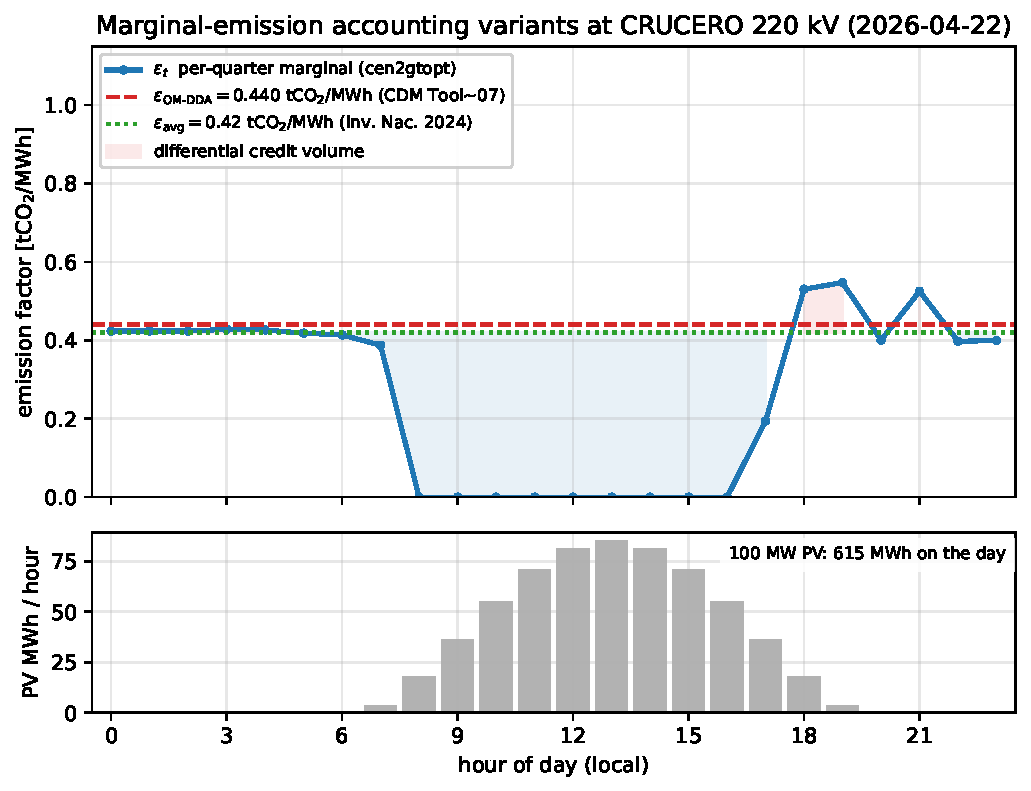
\includegraphics[width=\columnwidth]{figures/credits_curves.pdf}
\caption{24-hour overlay at CRUCERO 220~kV on 2026-04-22:
per-quarter $\varepsilon_t$ from \cenpipe{} (blue),
dispatch-weighted OM-DDA per~\eqref{eq:om-dda} (dashed red),
and the 2024 \textit{Inventario Nacional} national-average factor
(dotted green).  The shaded area between $\varepsilon_t$ and
$\varepsilon_{\mathrm{avg}}$ is the differential credit volume per
accounting choice; the lower bar trace shows the hypothetical 100~MW
PV plant's hourly energy injection.  Per-quarter values are taken
from cen2gtopt; the ten quarters without published
$\lambda^{\mathrm{CEN}}$ are linearly interpolated.}
\label{fig:credits-curves}
\end{figure}

\begin{table}[t]
\centering
\caption{Daily and annualised CO$_2$ credits for a hypothetical
100~MW PV at CRUCERO 220~kV under three accounting variants.
Annual figures are daily $\times 365$ without seasonality
correction; see~Sec.~\ref{sec:credits-limits}.}
\label{tab:credits-worked}
% credits_worked_example.tex
% Worked-example table: 100 MW hypothetical PV at CRUCERO 220 kV on
% 2026-04-22.  Daily figures are computed from
% /tmp/wp_marg_co2_figures/data_2026-04-22.parquet via the helper script
% figures/make_credits_curves.py; annual figures are the daily figures
% multiplied by 365 (no seasonal adjustment is applied — see
% Sec.~\ref{sec:credits-limits}).
\setlength{\tabcolsep}{4pt}
\renewcommand{\arraystretch}{1.10}
\begin{tabular}{@{}lrrr@{}}
\toprule
Accounting variant
  & $\bar\varepsilon$
  & Daily credit
  & Annual credit \\
  & [tCO$_2$/MWh]
  & [tCO$_2$/d]
  & [tCO$_2$/yr] \\
\midrule
$\varepsilon_t$, hourly-marginal (Art.~6.4 / EnergyTag) & 0.032$^{\dagger}$ & 19.9 & 7\,270 \\
$\varepsilon_{\mathrm{OM\text{-}DDA}}$, CDM Tool~07 OM       & 0.440 & 270.6 & 98\,785 \\
$\varepsilon_{\mathrm{simp\text{-}OM}}$, simplified OM (29-bus mean) & 0.241 & 148.4 & 54\,167 \\
$\varepsilon_{\mathrm{avg}}$, national grid (Inv. Nac.\ 2024) & 0.420 & 258.4 & 94\,306 \\
\midrule
$\Delta$ (OM-DDA $-$ hourly)        & --- &  +250.7 & +91\,515 \\
$\Delta$ (avg-grid $-$ OM-DDA)      & --- &  $-12.3$  & $-4\,479$  \\
\bottomrule
\end{tabular}

% $^\dagger$ effective time-matched mean for the chosen PV profile, computed
% as $\sum_h \mathrm{MWh}_h \cdot \varepsilon_h / \sum_h \mathrm{MWh}_h$;
% the per-quarter $\varepsilon_t$ itself ranges from 0 to
% 1.04~tCO$_2$/MWh (see Fig.~\ref{fig:credits-curves}).

\end{table}

The same comparison establishes the converse claim of
Sec.~\ref{sec:credits-ops}: a BESS sited at CRUCERO that times its
charging to the 09:00--16:00 window (when
$\varepsilon^{\mathrm{bus}}\approx 0$) and its discharging to the
18:00--23:00 window (when $\varepsilon^{\mathrm{bus}}\approx 0.5$
tCO$_2$/MWh) earns nearly the full $\Delta\varepsilon$ as ER per
discharged MWh — an effect entirely invisible to OM-DDA or
average-factor accounting and the central business case of
Sec.~\ref{sec:bess}.

\subsection{Limitations and Forward Agenda}
\label{sec:credits-limits}

Three structural caveats apply.  First, Tool~07 explicitly
disallows imports outside the project boundary and requires the
project boundary to coincide with a single synchronously
interconnected system; for the SEN — a single synchronous system
since the SIC/SING merger of 2017 — the criterion is satisfied, but
projects sited near future Argentine or Peruvian interconnections
will need re-examination.  Second, Verra has not yet endorsed
quarter-hourly granularity; the present paper positions itself as
forward-looking precedent and the cen2gtopt parquet schema is
designed to be aggregable to any coarser granularity an auditor
demands without recomputation.  Third, the $\hat\lambda$ and
$\hat\varepsilon^{\mathrm{bus}}$ produced by \cenpipe{} are
\emph{post-hoc} signals derived from the cleared dispatch; for
ex-ante crediting (forecast-based issuance) an additional
probabilistic layer would be needed.  A natural candidate is the
\texttt{gtopt} stochastic dual-dynamic programming engine
(see Sec.~\ref{sec:conclusions}), whose per-scenario per-stage
shadow prices on the energy-balance constraints would propagate
into a per-scenario forecast of $\varepsilon^{\mathrm{bus}}_{b,t}$.
A separate question — whether the carbon-credit issuance registry
should be a national entity (e.g.\ MAPS-Chile or
BIOCARBON~\cite{BiocarbonRegistry,MAPSChile}) or an international
one (Article~6.4 SBM) — is outside the scope of this paper.

The annualisation $\times 365$ used in
Table~\ref{tab:credits-worked} is a deliberate over-simplification:
the SEN exhibits strong seasonal hydrology and solar variability,
and the 2026-04-22 day is autumnal in the southern hemisphere with
above-average daytime solar marginal regime.  A multi-day
extension covering at least one full year is identified as the
priority next step; the cen2gtopt orchestrator already supports
multi-day Hive-partitioned output, and the worked-example pipeline
of Fig.~\ref{fig:credits-curves} is a pure function of its parquet
inputs.  Convergence of the daily-mean $\varepsilon^{\mathrm{bus}}_b$
to a season-stable annual factor is expected within
\SIrange{60}{90}{days} of cumulative dispatch coverage.
